\documentclass[border=5pt]{standalone}
\usepackage{graphicx}
\usepackage{tikz}

\renewcommand\familydefault{\sfdefault}

\usetikzlibrary{arrows.meta}
\usetikzlibrary{shapes.geometric}
\usetikzlibrary{positioning}
\usetikzlibrary{calc,quotes}
\usetikzlibrary{backgrounds}

\usetikzlibrary{shapes.misc}
\usetikzlibrary{shapes,decorations,shadows}
\usetikzlibrary{decorations.pathmorphing}
\usetikzlibrary{decorations.shapes}
\usetikzlibrary{fadings}
\usetikzlibrary{patterns}
\usetikzlibrary{calc}
\usetikzlibrary{shapes.gates.logic.IEC}
\usetikzlibrary{shapes.gates.logic.US}
\usetikzlibrary{fit,chains}
\usetikzlibrary{positioning}
\usepgflibrary{shapes}
\usetikzlibrary{scopes}

\pgfdeclarelayer{bg}    % declare background layer
\pgfdeclarelayer{bgone}    % declare background layer
\pgfsetlayers{bg,bgone,main}  % set the order of the layers (main is the standard layer)

\usepackage[shortlabels]{enumitem}
\setlist[enumerate]{nosep}
\usepackage{enumitem}
\usepackage{multicol}
\setlist[itemize]{noitemsep}

\begin{document}
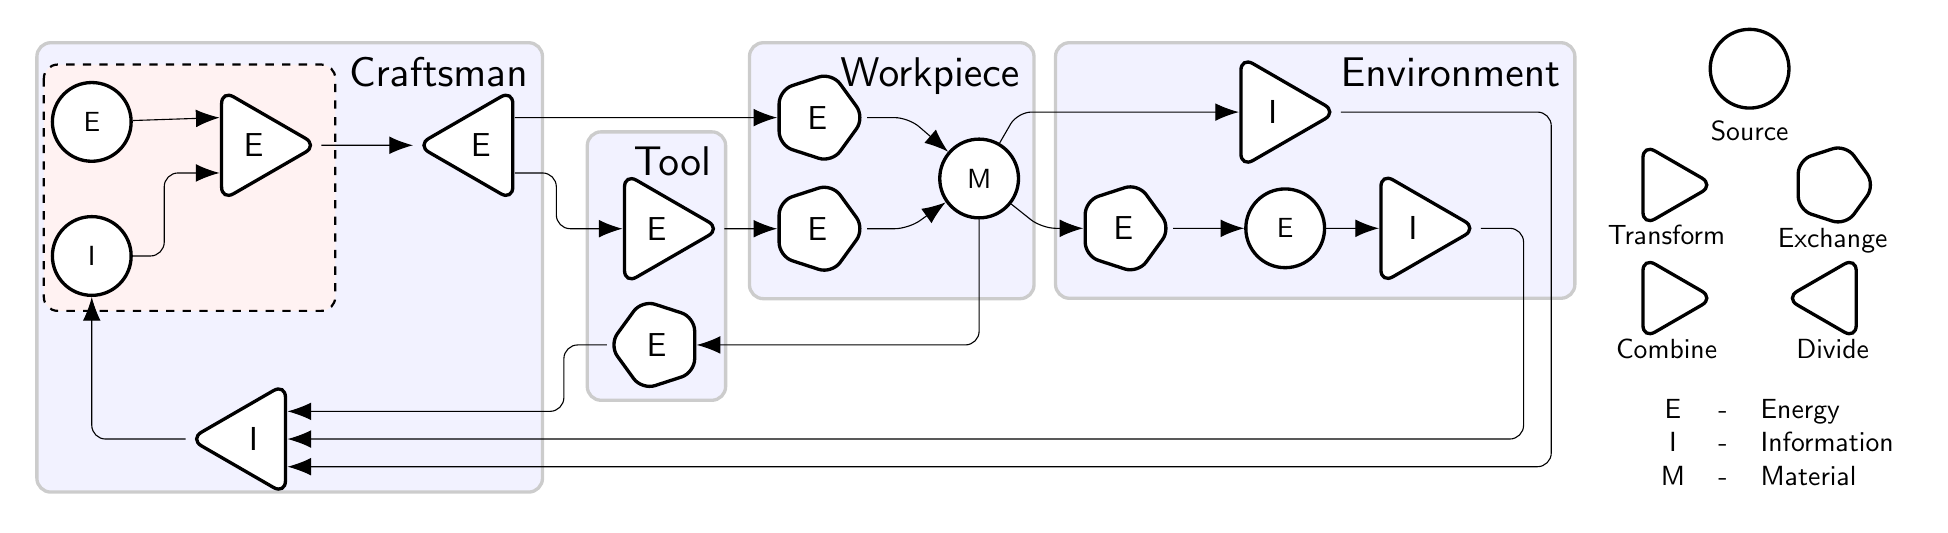
\begin{tikzpicture}[
T/.style={regular polygon, regular polygon sides=3,shape border rotate=90, draw=black, fill=white, very thick, minimum size=10mm,shape border rotate=270,scale=1.2},
E/.style={regular polygon, regular polygon sides=5,shape border rotate=90, draw=black, fill=white, very thick, minimum size=10mm,shape border rotate=270,scale=1.2},
C/.style={regular polygon, regular polygon sides=3,shape border rotate=90, draw=black, fill=white, very thick, minimum size=10mm,shape border rotate=270,scale=1.2},
D/.style={regular polygon, regular polygon sides=3,shape border rotate=270, draw=black, fill=white, very thick, minimum size=10mm,shape border rotate=90,scale=1.2},
S/.style={circle, draw=black, fill=white!5, very thick, minimum size=10mm},
ii/.style={-{Latex[length=3mm]}},
p/.style={circle, draw=red!95, fill=black, minimum size=2mm},
ii/.style={-{Latex[length=3mm]}},
ni/.style={-{Latex[length=3mm]},blue},
d/.style={dashed,-{Latex[length=3mm]},black!80},
blockU/.style={rectangle, draw=black, thick, fill=white,
      text width=8em, text centered},  rounded corners=0.5em,
blockC/.style={rectangle, draw=black, thick, fill=white,
      text width=8em, text centered,
      minimum height=4em},
blockL/.style={rectangle, draw=black, thick, fill=white,
      text width=10em, text ragged},
mynode/.style={regular polygon, regular polygon sides=3,draw=black,minimum size=10mm}
%squarednode/.style={rectangle, draw=red!60, fill=red!5, very thick, minimum size=5mm},
]
%
%\draw[help lines, color=gray!30, dashed] (0,0) grid (40,25);
%\draw[->,ultra thick] (0,0)--(20,0) node[below]{y};
%\draw[->,ultra thick] (0,0)--(0,10) node[above]{x};
%

% Nodes
\node[C] at (10, 10)                                         (C1) {E};
\node[S] [left of=C1, yshift=-4em, xshift=-3em]              (S1) {I};
\node[S] [above of=S1, left of=C1, yshift=-2em, xshift=-3em] (S2) {E};
\node[D] [right of=C1, xshift=4em]                           (D0p5) {E};
\node[] [right of=D0p5, xshift=3.5em, yshift=1em]            (T1) {};
\node[E] [right of=T1, xshift=2em, yshift=0em]              (E1) {E};
\node[S] [right of=E1, xshift=3em,yshift=-2.2em]             (S3) {M};
\node[T] [right of=S3, xshift=6em, yshift=2em]               (T3) {I};
\node[E] [right of=S3, xshift=1.5em, yshift=-1.5em]              (E2) {E};
\node[S] [right of=E2, xshift=3em]                           (S4) {E};
\node[T] [right of=S4, xshift=1em, yshift=0em]               (T4) {I};
\node[C] [below of=C1, yshift=-6em,shape border rotate=90]   (C2) {I};
\node[E] [below of=E1, yshift=-0.5em]                          (E3) {E};
\node[E] [below of=T1, yshift=-4em,shape border rotate=90]     (E4) {E};
\node[T] at (E4 |- E3) (T5) {E};
%

\node[S] [yshift=-1.5em, below of=K0] at (29,12.5)(K1) {};
\node[anchor=center, minimum height=5em, yshift=-0.75em]  at (K1.south) (Txt1) {Source};

\node[T] [anchor=north, xshift=-2.5em, yshift=-0.75em] at (Txt1) (K2) {};
\node[anchor=center, minimum height=5em, yshift=-0.75em]  at (K2.south) (Txt2) {Transform};

\node[E] [anchor=center, xshift=+2.5em,scale=0.9] at (K2-|Txt1) (K3) {};
\node[anchor=center, minimum height=5em,yshift=-0.2em]  at (Txt2-|K3) (Txt3) {Exchange};

\node[] at (Txt1 |- Txt2) (r2) {};

\node[C] [anchor=north, xshift=-2.5em, yshift=-1em] at (r2) (K4) {};
\node[anchor=center, minimum height=5em, yshift=-0.75em]  at (K4.south) (Txt4) {Combine};

\node[C] [anchor=north, xshift=2.5em, yshift=-1em, shape border rotate=90] at (r2) (K5) {};
\node[anchor=center, minimum height=5em, yshift=-0.75em]  at (K5.south) (Txt5) {Divide};

\node[] at (Txt1 |- Txt4) (r3) {};

\node[minimum height = 3em, yshift=-3.5em,xshift=1em] at (r3) (K0) {
\begin{tabular}{ccl}
E & - & Energy      \\
I & - & Information \\
M & - & Material   
\end{tabular}
};



% Paths
\draw[ii] (S1.east) -| ([yshift=-1em, xshift=-2em] C1.west) -- ([yshift=-1em] C1.west);
\draw[ii] (S2) -- ([yshift=1em] C1.west);
\draw[ii] (E1.east) -- ([xshift=1.5em] E1.east) -- (S3);
\draw[ii] (E3.east) -- ([xshift=1.5em] E3.east) -- (S3);
%\draw[ii] (E1) -- (S3);
\draw[ii] (S3) -- ([xshift=-8em] T3.west) -- (T3);
\draw[ii] (S3) -- ([xshift=-1.5em] E2.west) -- (E2);
\draw[ii] (E2) -- (S4);
\draw[ii] (S4) -- (T4);
\draw[ii] (C2) -| (S1);
% See https://stuff.mit.edu/afs/athena/contrib/tex-contrib/beamer/pgf-1.01/doc/generic/pgf/version-for-tex4ht/en/pgfmanualse11.html

\draw[ii] (C1) -- (D0p5);
%\draw[ii] ([yshift=1em] D0p5.east) -- ([yshift=1em, xshift=1.5em] D0p5.east) |- (T1);
\draw[ii] ([yshift=1em] D0p5.east) -- (E1);
\draw[ii] ([yshift=-1em] D0p5.east) -- ([yshift=-1em, xshift=1.5em] D0p5.east) |- (T5);

\draw[ii] (T5) -- (E3);

\draw[ii] (S3) |- (E4);

%    Manufacturing \\
%    Pattern\\
%    \end{tabular}};

\node[yshift=1em,xshift=3em] at (C2 -| D0p5) (p1) {};
\node[yshift=0em,xshift=4em] at (C2 -| T4) (p2) {};
\node[yshift=-1em,xshift=5em] at (C2 -| T4) (p3) {};


\draw[ii] (E4.west) -| (p1.center) -- ([yshift=1em] C2.east);
\draw[ii] (T4.east) -| (p2.center) -- ([yshift=0em] C2.east);
\draw[ii] (T3.east) -| (p3.center) -- ([yshift=-1em] C2.east);

%% Background Areas
\begin{pgfonlayer}{bg}    % select the background layer
    
   
\node[yshift=1em] at (T1.north) (T2) {};

\node[yshift=1em, xshift=1em] at (T2.north -| D0p5.east) (crafttr) {};
\node[yshift=-0.5em, xshift=-0.5em] at ( C2.south -|  S1.west) (craftbl) {};
\filldraw[color=black!20, fill=blue!5, very thick, rounded rectangle] (craftbl) rectangle (crafttr);

\node[yshift=3.5em, xshift=2.5em] at (T5) (tooltr) {};
\node[yshift=-2em, xshift=-2.5em] at (E4) (toolbl) {};
\filldraw[color=black!20, fill=blue!5, very thick, rounded rectangle] (tooltr) rectangle (toolbl);

\node[yshift=1em, xshift=0.5em] at (T2.north -| S3.east) (Worktr) {};
\node[yshift=-1em, xshift=-1em] at (E3.south -|  E1.west) (Workbl) {};
\filldraw[color=black!20, fill=blue!5, very thick, rounded rectangle] (Workbl) rectangle (Worktr);

\node[yshift=1em, xshift=0.5em] at (T2.north -| p3.east) (Envirotr) {};
\node[yshift=-1em, xshift=-1em] at (E2.south -|  E2.west) (Envirobl) {};
\filldraw[color=black!20, fill=blue!5, very thick, rounded rectangle] (Envirotr) rectangle (Envirobl);

\end{pgfonlayer}
%% Text
\node[text width = 10em, anchor=north east, align=right, scale=1.5] at (crafttr) {Craftsman};
\node[text width = 10em, anchor=north east, align=right, scale=1.5] at (tooltr) {Tool};
\node[text width = 10em, anchor=north east, align=right, scale=1.5] at (Worktr) {Workpiece};
\node[text width = 10em, anchor=north east, align=right, scale=1.5] at (Envirotr) {Environment};



\node[xshift=-0.25em, yshift=1.5em] at (C1.north -| S1.west) (PBox1) {};
\node[xshift=0.5em, yshift=-0.5em] at (S1.south -| C1.east) (PBox2) {};
%	
\begin{pgfonlayer}{bgone}    % select the background layer
	\filldraw[fill=red!5, draw=black, thick, dashed] (PBox1) rectangle (PBox2);
%	
\end{pgfonlayer}




\end{tikzpicture}
\end{document}